% Options for packages loaded elsewhere
\PassOptionsToPackage{unicode}{hyperref}
\PassOptionsToPackage{hyphens}{url}
%
\documentclass[
]{article}
\usepackage{amsmath,amssymb}
\usepackage{iftex}
\ifPDFTeX
  \usepackage[T1]{fontenc}
  \usepackage[utf8]{inputenc}
  \usepackage{textcomp} % provide euro and other symbols
\else % if luatex or xetex
  \usepackage{unicode-math} % this also loads fontspec
  \defaultfontfeatures{Scale=MatchLowercase}
  \defaultfontfeatures[\rmfamily]{Ligatures=TeX,Scale=1}
\fi
\usepackage{lmodern}
\ifPDFTeX\else
  % xetex/luatex font selection
\fi
% Use upquote if available, for straight quotes in verbatim environments
\IfFileExists{upquote.sty}{\usepackage{upquote}}{}
\IfFileExists{microtype.sty}{% use microtype if available
  \usepackage[]{microtype}
  \UseMicrotypeSet[protrusion]{basicmath} % disable protrusion for tt fonts
}{}
\makeatletter
\@ifundefined{KOMAClassName}{% if non-KOMA class
  \IfFileExists{parskip.sty}{%
    \usepackage{parskip}
  }{% else
    \setlength{\parindent}{0pt}
    \setlength{\parskip}{6pt plus 2pt minus 1pt}}
}{% if KOMA class
  \KOMAoptions{parskip=half}}
\makeatother
\usepackage{xcolor}
\usepackage[margin=1in]{geometry}
\usepackage{color}
\usepackage{fancyvrb}
\newcommand{\VerbBar}{|}
\newcommand{\VERB}{\Verb[commandchars=\\\{\}]}
\DefineVerbatimEnvironment{Highlighting}{Verbatim}{commandchars=\\\{\}}
% Add ',fontsize=\small' for more characters per line
\usepackage{framed}
\definecolor{shadecolor}{RGB}{248,248,248}
\newenvironment{Shaded}{\begin{snugshade}}{\end{snugshade}}
\newcommand{\AlertTok}[1]{\textcolor[rgb]{0.94,0.16,0.16}{#1}}
\newcommand{\AnnotationTok}[1]{\textcolor[rgb]{0.56,0.35,0.01}{\textbf{\textit{#1}}}}
\newcommand{\AttributeTok}[1]{\textcolor[rgb]{0.13,0.29,0.53}{#1}}
\newcommand{\BaseNTok}[1]{\textcolor[rgb]{0.00,0.00,0.81}{#1}}
\newcommand{\BuiltInTok}[1]{#1}
\newcommand{\CharTok}[1]{\textcolor[rgb]{0.31,0.60,0.02}{#1}}
\newcommand{\CommentTok}[1]{\textcolor[rgb]{0.56,0.35,0.01}{\textit{#1}}}
\newcommand{\CommentVarTok}[1]{\textcolor[rgb]{0.56,0.35,0.01}{\textbf{\textit{#1}}}}
\newcommand{\ConstantTok}[1]{\textcolor[rgb]{0.56,0.35,0.01}{#1}}
\newcommand{\ControlFlowTok}[1]{\textcolor[rgb]{0.13,0.29,0.53}{\textbf{#1}}}
\newcommand{\DataTypeTok}[1]{\textcolor[rgb]{0.13,0.29,0.53}{#1}}
\newcommand{\DecValTok}[1]{\textcolor[rgb]{0.00,0.00,0.81}{#1}}
\newcommand{\DocumentationTok}[1]{\textcolor[rgb]{0.56,0.35,0.01}{\textbf{\textit{#1}}}}
\newcommand{\ErrorTok}[1]{\textcolor[rgb]{0.64,0.00,0.00}{\textbf{#1}}}
\newcommand{\ExtensionTok}[1]{#1}
\newcommand{\FloatTok}[1]{\textcolor[rgb]{0.00,0.00,0.81}{#1}}
\newcommand{\FunctionTok}[1]{\textcolor[rgb]{0.13,0.29,0.53}{\textbf{#1}}}
\newcommand{\ImportTok}[1]{#1}
\newcommand{\InformationTok}[1]{\textcolor[rgb]{0.56,0.35,0.01}{\textbf{\textit{#1}}}}
\newcommand{\KeywordTok}[1]{\textcolor[rgb]{0.13,0.29,0.53}{\textbf{#1}}}
\newcommand{\NormalTok}[1]{#1}
\newcommand{\OperatorTok}[1]{\textcolor[rgb]{0.81,0.36,0.00}{\textbf{#1}}}
\newcommand{\OtherTok}[1]{\textcolor[rgb]{0.56,0.35,0.01}{#1}}
\newcommand{\PreprocessorTok}[1]{\textcolor[rgb]{0.56,0.35,0.01}{\textit{#1}}}
\newcommand{\RegionMarkerTok}[1]{#1}
\newcommand{\SpecialCharTok}[1]{\textcolor[rgb]{0.81,0.36,0.00}{\textbf{#1}}}
\newcommand{\SpecialStringTok}[1]{\textcolor[rgb]{0.31,0.60,0.02}{#1}}
\newcommand{\StringTok}[1]{\textcolor[rgb]{0.31,0.60,0.02}{#1}}
\newcommand{\VariableTok}[1]{\textcolor[rgb]{0.00,0.00,0.00}{#1}}
\newcommand{\VerbatimStringTok}[1]{\textcolor[rgb]{0.31,0.60,0.02}{#1}}
\newcommand{\WarningTok}[1]{\textcolor[rgb]{0.56,0.35,0.01}{\textbf{\textit{#1}}}}
\usepackage{longtable,booktabs,array}
\usepackage{calc} % for calculating minipage widths
% Correct order of tables after \paragraph or \subparagraph
\usepackage{etoolbox}
\makeatletter
\patchcmd\longtable{\par}{\if@noskipsec\mbox{}\fi\par}{}{}
\makeatother
% Allow footnotes in longtable head/foot
\IfFileExists{footnotehyper.sty}{\usepackage{footnotehyper}}{\usepackage{footnote}}
\makesavenoteenv{longtable}
\usepackage{graphicx}
\makeatletter
\newsavebox\pandoc@box
\newcommand*\pandocbounded[1]{% scales image to fit in text height/width
  \sbox\pandoc@box{#1}%
  \Gscale@div\@tempa{\textheight}{\dimexpr\ht\pandoc@box+\dp\pandoc@box\relax}%
  \Gscale@div\@tempb{\linewidth}{\wd\pandoc@box}%
  \ifdim\@tempb\p@<\@tempa\p@\let\@tempa\@tempb\fi% select the smaller of both
  \ifdim\@tempa\p@<\p@\scalebox{\@tempa}{\usebox\pandoc@box}%
  \else\usebox{\pandoc@box}%
  \fi%
}
% Set default figure placement to htbp
\def\fps@figure{htbp}
\makeatother
\setlength{\emergencystretch}{3em} % prevent overfull lines
\providecommand{\tightlist}{%
  \setlength{\itemsep}{0pt}\setlength{\parskip}{0pt}}
\setcounter{secnumdepth}{-\maxdimen} % remove section numbering
\renewcommand{\figurename}{Figura}
\renewcommand{\tablename}{Tabla}
\usepackage{float}
\floatplacement{figure}{H}
\usepackage{titling}
\usepackage{lipsum}
\usepackage{fancyhdr}
\usepackage{etoolbox}
\usepackage{setspace}
\usepackage{titlesec}
\usepackage{emptypage}
\pagestyle{fancy}
\usepackage{placeins}
\fancyhf{}
\patchcmd{\maketitle}{\@maketitle}{\centering\vspace*{4cm}\@maketitle}{}{}
\thispagestyle{empty}
\usepackage{booktabs}
\usepackage{longtable}
\usepackage{array}
\usepackage{multirow}
\usepackage{wrapfig}
\usepackage{float}
\usepackage{colortbl}
\usepackage{pdflscape}
\usepackage{tabu}
\usepackage{threeparttable}
\usepackage{threeparttablex}
\usepackage[normalem]{ulem}
\usepackage{makecell}
\usepackage{xcolor}
\usepackage{bookmark}
\IfFileExists{xurl.sty}{\usepackage{xurl}}{} % add URL line breaks if available
\urlstyle{same}
\hypersetup{
  hidelinks,
  pdfcreator={LaTeX via pandoc}}

\author{}
\date{\vspace{-2.5em}}

\begin{document}

\begin{titlepage}
\centering
\vspace*{4cm} % espacio superior

{\Huge \textbf{Trabajo práctico 2 Estadística Bayesiana}}\\[2cm]

{\Large Agustina Roura}\\[0.5cm]
{\Large Cristian Nahuel Coveñas}\\[0.5cm]
{\Large Juan Sebastian Reines}\\[2cm]

{\large Fecha: Mayo 2025}

\vfill

\end{titlepage}

\newpage

\section{Introducción}\label{introducciuxf3n}

El ozono \((O_3)\), una molécula de tres átomos de oxígeno, exhibe una
fascinante dualidad en su comportamiento y efectos. En las capas
superiores de la atmósfera, conforma la vital capa de ozono, un escudo
protector que filtra la radiación ultravioleta del sol, permitiendo la
vida tal como la conocemos. Sin embargo, a nivel de la superficie
terrestre, este mismo gas se transforma en un contaminante atmosférico
de considerable impacto negativo, afectando la salud humana a través de
la irritación del sistema respiratorio y ocular, el desencadenamiento de
episodios de asma y el deterioro de la función pulmonar. Además, su
presencia en el aire urbano contribuye al smog y puede causar daños
significativos en la vegetación.

Ante la creciente preocupación por los efectos del ozono a nivel del
suelo, Brian Tarkington, investigador del California Primate Research
Center, llevó a cabo un estudio con el objetivo de cuantificar su
impacto en el desarrollo de organismos vivos. Específicamente, se
propuso investigar si la exposición a un ambiente enriquecido con ozono
afectaba el crecimiento de ratas jóvenes. Para ello, diseñó un
experimento controlado donde un grupo de 46 ratas de la misma edad
fueron divididas aleatoriamente en dos subgrupos iguales. Uno de estos
grupos fue expuesto a un ambiente con alta concentración de ozono,
mientras que el otro se mantuvo en un ambiente libre de este gas. Tras
un período de siete días, se registró la diferencia en el peso de cada
animal, generando un conjunto de datos que permite analizar
comparativamente el efecto de la exposición al ozono.

Con el objetivo de dar respuesta a la inquietud de Tarkington, abordaremos
el problema mediante el uso modelos bayesianos. En particular, consideramos
dos modelos probabilísticos con sutiles diferencias en su formulación.

El primer modelo propuesto para modelizar el cambio en el peso de las ratas
en cada grupo se modeliza con una distribución normal, permitiendo medias
\((\mu_O,\ \mu_C)\) y varianzas \((\sigma_O^2,\ \sigma_C^2)\) específicas para
cada grupo.

El segundo modelo propuesto, en contraste, emplea la distribución T
de Student con 3 grados de libertad \((v = 3)\), esta alternativa
resulta especialmente útil cuando se desea robustez frente a posibles
valores atípicos o colas pesadas en la distribución de los datos.

Más allá de la comparación de estos modelos y la respuesta a la pregunta
de investigación sobre el efecto del ozono, el objetivo principal del
estudio es profundizar el uso del algoritmo de Metropolis-Hastings (MH)
como un método de la inferencia bayesiana. Este algoritmo se vuelve
esencial cuando la distribución de probabilidad a posteriori de los
parámetros de interés no tiene una forma analítica conocida, lo que
dificulta la obtención directa de medidas de resúmenes o la realización
de inferencias. En esencia, el algoritmo de Metropolis-Hastings funciona
como un proceso iterativo que genera una secuencia de valores (una
cadena de Markov) que, bajo ciertas condiciones, converge a la
distribución a posteriori deseada. Partiendo de un valor inicial para
los parámetros, el algoritmo sugiere un nuevo valor \(propuesto\) basado
en una distribución conocida. Este nuevo valor es luego aceptado o
rechazado según una probabilidad \(\alpha\) que depende de la razón entre
la verosimilitud de los datos bajo el nuevo valor de los parámetros y la
verosimilitud bajo el valor actual, multiplicada por la razón de las
probabilidades a priori de los dos valores.

\[\alpha = \min \left\{ 1, \frac{p(y')q(y^{(t)} | y')}{p(y^{(t)})q(y' | y^{(t)})} \right\}\]

Si el valor \(propuesto\) tiene una mayor probabilidad a posteriori (o una
probabilidad no mucho menor), es más probable que sea aceptado. Si es
rechazado, el valor actual se mantiene para la siguiente iteración. Tras
un número suficiente de iteraciones, las muestras generadas por el
algoritmo se aproxima a la distribución del \(posterior\) objetivo y asi
calcular diversas cantidades de interés, como medias, medianas,
intervalos de credibilidad, etc. La clave del algoritmo radica en la
elección adecuada de la distribución de propuesta para asegurar una
exploración eficiente del espacio de parámetros y una rápida
convergencia a la distribución objetivo.

\newpage

\section{Primeros pasos en Metropolis-Hastings}\label{Objetivo-1}

El algoritmo de Metropolis-Hastings, implementado en escala logarítmica,
constituye una herramienta robusta para obtener muestras del
\(posterior\). Sin embargo, su aplicación directa a modelos complejos
puede ser desafiante sin una sólida comprensión de sus fundamentos y
técnicas asociadas. Como preparación para la aplicación del algoritmo de
Metropolis-Hastings a modelos bayesianos más complejos, se llevó a cabo
una exploración inicial del algoritmo en escenarios más simples.

Se comenzó con un escenario donde \(X\) es la variable aleatoria
de interés, cuya función de densidad corresponde a una distribución
Gamma con parámetros \(\alpha = 3\) y \(\beta = 2\) (\(X \sim Gamma(3,2)\)).

\begin{figure}

{\centering \includegraphics{TP-2---El-Dibu-de-la-vida_files/figure-latex/f1-1} 

}

\caption{Distribucion de densidad de X}\label{fig:f1}
\end{figure}

La Figura \ref{fig:f1} ilustra la forma de la distribución de densidad
de la variable aleatoria \(X\).

A continuación, se propuso encontrar la función de densidad de una nueva
variable aleatoria \(Y=log(X)\). Para ello, recurrimos a la técnica de
transformación de variables de la siguiente manera:

\(\text{Sea }Y = g(X) = log(x) \text{, donde la función } g:(0,\ +\infty) \rightarrow \mathbb{R}.\)

\(\text{Su función inversa es: }g^{-1}(X) = e^{X} \text{, con dominio } g^{-1}: \mathbb{R} \rightarrow (0,\ +\infty).\)

Luego, la función de densidad de \(Y\), \(P_Y(y)\), se obtiene a partir de
la función de densidad \(X\), \(P_X(x)\), utilizando la siguiente relación:
\vspace{0cm}
\[P_Y(y) = P_X(g^{-1}(y)) \left| \frac{d}{dy} g^{-1}(y) \right|\]
\(\text{Sustituyendo } g^{-1}(y) = e^{y}, \text{ obtenemos:}\)
\vspace{0cm}
\[P_Y(y) = P_X(e^{y}) \left| \frac{d}{dy} e^{y} \right| = P_X(e^{y})\left| e^{y} \right|\]

\newpage

\(\text{De esta forma podemos graficar la función de densidad de } Y = log(X)\)

\begin{figure}

{\centering 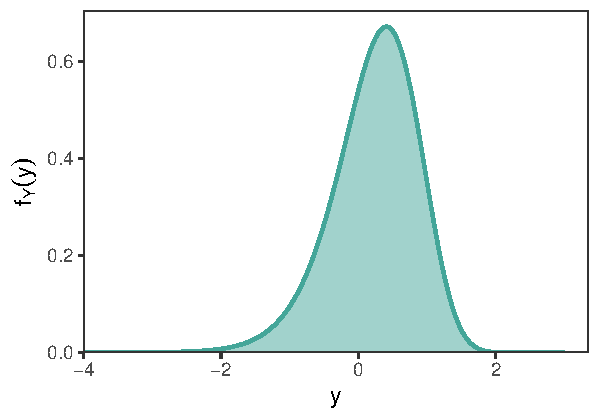
\includegraphics{TP-2---El-Dibu-de-la-vida_files/figure-latex/f2-1} 

}

\caption{Distribucion de densidad de Y = log(X)}\label{fig:f2}
\end{figure}

Dadas las funciones de densidad para las variables \(X\) e \(Y=log(X)\), tal
como se ilustra en las Figuras \ref{fig:f1} y \ref{fig:f2}
respectivamente, se consideró la aplicación del algoritmo de
Metropolis-Hastings para generar 10000 muestras de \(X\). Si bien la
distribución normal suele ser una elección inicial conveniente para
generar propuestas de nuevos valores en el algoritmo de
Metropolis-Hastings, su aplicación en espacios paramétricos acotados
puede resultar ineficiente debido al incremento en la tasa de rechazo
generado por propuestas fuera del dominio, lo que ralentiza la
exploración del espacio paramétrico y la convergencia del algoritmo.

Porlo que se optó por realizar el proceso de muestreo sobre la variable
transformada \(Y=log(X)\), utilizando una distribución normal como función
de propuesta, con una desviación estándar \(\sigma = 0.2\) y centrada en
un valor inicial de \(\mu = 0\). Esta estrategia de trabajar en un espacio
no acotado permitió seguir utilizando las propiedades convenientes de la
distribución normal como propuesta.

\begin{figure}

{\centering \includegraphics{TP-2---El-Dibu-de-la-vida_files/figure-latex/f3-1} 

}

\caption{Histograma de la muestras de Y = log(X)}\label{fig:f3}
\end{figure}

\begin{figure}

{\centering \includegraphics{TP-2---El-Dibu-de-la-vida_files/figure-latex/f4-1} 

}

\caption{Traceplot de la muestras de Y = log(X)}\label{fig:f4}
\end{figure}

Luego de la aplicación del método, como se puede observar en la Figura
\ref{fig:f3}, las muestras obtenidas presentan una semejanza notable con
la distribución objetivo. Además como se puede observar en la Figura
\ref{fig:f4} (trace plot) revela una baja autocorrelación en las cadenas
de Markov generadas. Esto sugiere un buen ajuste del algoritmo de
Metropolis-Hastings, resultado de su aplicación sobre la variable aleatoria Y,
cuyo dominio resultó apropiado para la distribución de propuesta utilizada.

Para una evaluación más exhaustiva de la calidad del ajuste del método
implementado, se calcularon las medidas de diagnóstico sobre la distribución
propuesta utilizada para generar la muestra.

\begin{figure}

{\centering \includegraphics{TP-2---El-Dibu-de-la-vida_files/figure-latex/f5-1} 

}

\caption{Traceplots con sigma = 0.2}\label{fig:f5}
\end{figure}

\begin{table}[H]
\centering
\caption{\label{tab:t1}Medidas de Diagnóstico del Algoritmo Metropolis-Hastings}
\centering
\begin{tabular}[t]{l>{\raggedleft\arraybackslash}p{3cm}}
\toprule
Métrica & Valor\\
\midrule
$\hat{R}$ & 1.001601\\
$N_{eff}$ Cadena 1 & 205.383136\\
$N_{eff}$ Cadena 2 & 204.745440\\
$N_{eff}$ Cadena 3 & 212.588630\\
$N_{eff}$ Cadena 4 & 188.515861\\
\addlinespace
$N_{eff}$ Total & 811.233067\\
\bottomrule
\end{tabular}
\end{table}

El análisis visual del trace plot, presentado en la Figura \ref{fig:f5}, sugiere una convergencia de las cuatro cadenas de Markov hacia una distribución común, lo que es consistente con el valor de \(\hat{R}\) de 1.001601, cercano al valor ideal de 1 que indica una buena mezcla entre las cadenas. No obstante, al examinar el tamaño efectivo de muestra (\(N_{eff}\)) presentado en la Tabla 1, se observa que los valores para cada cadena y el total son considerablemente bajos en relación con el número total de iteraciones. Este reducido tamaño efectivo de muestra indica una alta autocorrelación dentro de las cadenas. En consecuencia, la alta autocorrelación compromete la validez de utilizar directamente estas muestras para realizar inferencias precisas sobre la distribución objetivo.

Se continuó el análisis realizando el mismo procedimiento evaluando los resultados de las medidas de diagnóstico \(\hat{R}\) y \(N_{eff}\) , a través de diferentes valores de sigma.

\begin{figure}

{\centering \includegraphics{TP-2---El-Dibu-de-la-vida_files/figure-latex/f6-1} 

}

\caption{Traceplots con sigma = 1.3}\label{fig:f6}
\end{figure}

\begin{table}[H]
\centering
\caption{\label{tab:t2}Medidas de Diagnóstico del Algoritmo Metropolis-Hastings}
\centering
\begin{tabular}[t]{l>{\raggedleft\arraybackslash}p{3cm}}
\toprule
Métrica & Valor\\
\midrule
$\hat{R}$ & 1.000039\\
$N_{eff}$ Cadena 1 & 2062.416579\\
$N_{eff}$ Cadena 2 & 2016.848469\\
$N_{eff}$ Cadena 3 & 2115.095549\\
$N_{eff}$ Cadena 4 & 2087.321276\\
\addlinespace
$N_{eff}$ Total & 8281.681873\\
\bottomrule
\end{tabular}
\end{table}

Por lo que tomando en consideración dicho análisis se concluyó, como se puede observar en la Figura \ref{fig:f6}, que el valor de \(\sigma = 1.3\) parece ser el más adecuado para realizar inferencias ya que su valor de \(\hat{R}\) fue el más cercano a 1 de los comparados y las muestras de las diferentes cadenas se mezclas y parecen generar muestras representativas de la distribución objetivo ya que se estabilizan y muestran una buena mezcla. Además, el tamaño efectivo de muestra total fue el mayor, lo que señala que la autocorrelación es baja, y la menor de todas las comparadas. Por lo que se decidió continuar el análisis con un valor de \(\sigma = 1.3\) para la distribución propuesta. También se consideró apropiado no eliminar las primeras 1000 muestras ya que las cadenas de markov parecieran converger rápidamente a la misma distribución, lo que indica una elección apropiada del valor inicial.

Se implementó entonces la distribución propuesta normal centrada en 0, con \(\sigma = 1.3\), para obtener muestras de la variable X por medio del algoritmo Metropolis Hastings.

\begin{figure}

{\centering \includegraphics{TP-2---El-Dibu-de-la-vida_files/figure-latex/f7-1} 

}

\caption{Histograma de la muestras de X}\label{fig:f7}
\end{figure}

\begin{figure}

{\centering \includegraphics{TP-2---El-Dibu-de-la-vida_files/figure-latex/f8-1} 

}

\caption{Traceplot de la muestras de X}\label{fig:f8}
\end{figure}

Como se puede observar en la Figura \ref{fig:f7}, la muestras obtenidas del \(posterior\) con una distribución propuesta sugieren una buena aproximacion de la densidad teorica. Adicionalmente, en la Figura \ref{fig:f8}, se muestra un patrón de ruido blanco, lo que parece señalar una pérdida bastante rápida de la dependencia de cada muestra con la anterior. En resumen, las muestras tienen menos autocorrelación.

\subsection{Escala logarítmica}\label{escala-logaruxedtmica}

La implementación efectiva del algoritmo de Metropolis-Hastings, se enfrenta a desafíos computacionales relacionados con la magnitud de los números involucrados. Un obstáculo surge al evaluar la función de densidad objetivo en cada iteración del algoritmo. Esta función, que guía el proceso de muestreo hacia las regiones de mayor probabilidad, puede implicar la multiplicación de numerosos términos, especialmente cuando se modelan datos con múltiples observaciones. Si estos términos son pequeños, su producto puede rápidamente volverse tan pequeño que la computadora lo representa como cero, es decir se produce el fenómeno conocido como underflow. Este fenómeno dificulta la correcta ejecución del algoritmo de Metropolis-Hastings ya que puede conducir a errores que interrumpen el proceso de muestreo, impidiendo la obtención de las muestras necesarias para realizar inferencias válidas. Incluso si el programa no se detiene, un underflow puede resultar en la aceptación o rechazo incorrecto de valores propuestos, desviando la cadena de Markov de la distribución objetivo real y disminuyendo la fiabilidad de los resultados. Además, como el algoritmo evalúa la densidad objetivo en diferentes puntos del espacio paramétrico, la probabilidad de encontrar estas situaciones problemáticas se multiplica.

Una solución práctica es el uso de la escala logarítmica, al trabajar con los logaritmos de las probabilidades en lugar de las probabilidades directas, las operaciones de multiplicación se convierten en sumas y las divisiones se transforman en restas. Lo cual evita la utilización de números extremadamente pequeños, estabilizando los cálculos dentro del algoritmo de Metropolis-Hastings.

\newpage

A continuación, se implementó con el método de metropolis hastings en escala logarítmica la obtención de muestras de la variable X.

\begin{figure}

{\centering \includegraphics{TP-2---El-Dibu-de-la-vida_files/figure-latex/f9-1} 

}

\caption{Histograma de la muestras de X}\label{fig:f9}
\end{figure}

\begin{figure}

{\centering \includegraphics{TP-2---El-Dibu-de-la-vida_files/figure-latex/f10-1} 

}

\caption{Traceplot de la muestras de X}\label{fig:f10}
\end{figure}

\begin{figure}

{\centering \includegraphics{TP-2---El-Dibu-de-la-vida_files/figure-latex/f11-1} 

}

\caption{Traceplots con sigma = 1.3}\label{fig:f11}
\end{figure}

\begin{table}[H]
\centering
\caption{\label{tab:t3}Medidas de Diagnóstico del Algoritmo Metropolis-Hastings}
\centering
\begin{tabular}[t]{l>{\raggedleft\arraybackslash}p{3cm}}
\toprule
Métrica & Valor\\
\midrule
$\hat{R}$ & 1.000039\\
$N_{eff}$ Cadena 1 & 2062.416579\\
$N_{eff}$ Cadena 2 & 2016.848469\\
$N_{eff}$ Cadena 3 & 2115.095549\\
$N_{eff}$ Cadena 4 & 2087.321276\\
\addlinespace
$N_{eff}$ Total & 8281.681873\\
\bottomrule
\end{tabular}
\end{table}

La Figura \ref{fig:f9} muestra el histograma de las muestras obtenidas para la variable X, indicando una buena cobertura de su rango de variabilidad. El traceplot correspondiente a la Figura \ref{fig:f11} sugiere convergencia de las cadenas de markov hacia una misma distribución. Es notable que las medidas de diagnóstico (\(\hat{R}\) y \(N_{eff}\)) para estas muestras, mostradas en la Tabla 3, son idénticas a las calculadas previamente para la variable Y (Tabla 2 de la \ref{fig:f6}). Esta coincidencia sucede ya que, el algoritmo de Metropolis-Hastings se implementó utilizando cálculos en escala logarítmica para la estabilidad numérica para su optimización, las muestras generadas de la variable X se obtienen a partir del mismo valor de inicio, y por lo tanto sus propiedades de convergencia y eficiencia evaluadas por \(\hat{R}\) y \(N_{eff}\), permanecen inalteradas.

\newpage

\section{Inferencia Bayesiana en Múltiples Dimensiones}\label{Objetivo-2}

En modelos bayesianos con múltiples parámetros, la distribución a posteriori conjunta se vuelve el objetivo de inferencia. En este caso, la distribución objetivo tiene múltiples dimensiones y se obtiene mediante la aplicación de la regla de Bayes.

\subsubsection{Modelo Estadístico:}\label{modelo-estaduxedstico}

\vspace{-1.6cm}
\begin{center}
\begin{align*}
Y_i &\sim \text{Normal}(\mu, \sigma^2), \text{ con } i = 1, \dots, N \\
\mu &\sim \text{Normal}(0, 1^2) \\
\sigma &\sim \text{Gamma}(\alpha = 2, \beta = 2)
\end{align*}
\end{center}

La distribución a posteriori conjunta de los parámetros \(\theta = \{\mu, \sigma\}\) dado los datos \(y\) se obtiene mediante la regla de Bayes:
\[p(\mu, \sigma | y) = \frac{p(y | \mu, \sigma). p(\mu, \sigma)}{p(y)} \propto p( \boldsymbol{y}  \text{ | } \mu, \ \sigma).p(\mu, \ \sigma)\]
donde \(p(y | \mu, \sigma)\) es la verosimilitud de los datos dado los parámetros, \(p(\mu, \sigma) = p(\mu) p(\sigma)\) es la distribución a priori conjunta de los parámetros (asumiendo independencia entre \(\mu\) y \(\sigma\)).

La distribución a priori conjunta es el producto de las distribuciones a priori individuales:
\[p(\mu, \sigma) = p(\mu) . p(\sigma)\]

\subsubsection{Transformación a Espacio No Acotado}\label{transformaciuxf3n-a-espacio-no-acotado}

Un posible problema para la deducción analítica del posterior es el dominio de \(\sigma\) (\(\mathbb{R}^+\)). Para facilitar el muestreo o la optimización, a menudo se realiza una transformación a un espacio no acotado. En este caso, se propone la transformación \(\theta^* = \{\mu, \log(\sigma)\} \in \mathbb{R} \times \mathbb{R}\).

La relación entre \(\sigma\) y \(\sigma^*\) es \(\sigma = \exp(\sigma^*)\)

\subsubsection{Función de Densidad del Posterior Transformado}\label{funciuxf3n-de-densidad-del-posterior-transformado}

La función de densidad del posterior en el espacio transformado resulta:

\[p(\mu, \sigma^* \mid y) \propto p_y(y \mid \mu, \sigma^*).p_\mu(\mu).p_\sigma^*(\sigma^*)\]
\[\text{Teniendo en cuando la transformacion de }\sigma^* \text{ tenemos:}\]
\[p_\sigma^*(\sigma^*) = p_\sigma^*(g^1 (\sigma^*)) \left| \dfrac{d}{d\sigma^*} (g^1 (\sigma^*)) \right| \ = \ p_\sigma^*(exp(\sigma^*)).\exp(\sigma^*) \]
\[\text{De esta forma la función de densidad del posterior trasnformado resulta:}\]
\[p(\mu, \sigma^* \mid y) \propto\left[ \prod_{i = 1}^{N} p_y(y_i \mid \mu,\exp(\sigma^*))\right].p_\mu(\mu).p_\sigma^*(exp(\sigma^*)).\exp(\sigma^*)\]
\[\text{Aplicando logarítmo resulta:}\]
\[log\ p(\mu, \sigma^* \mid y) \propto\left[ \sum_{i = 1}^{N} log\ p_y(y_i \mid \mu,\exp(\sigma^*))\right]+log\ p_\mu(\mu)+log\ p_\sigma^*(exp(\sigma^*))+ \sigma^*\]

\newpage

\subsubsection{Implementación en R}\label{implementaciuxf3n-en-r}

\begin{Shaded}
\begin{Highlighting}[]
\CommentTok{\# Función de densidad posterior en escala logarítmica (sin normalizar)}
\NormalTok{log\_posterior }\OtherTok{\textless{}{-}} \ControlFlowTok{function}\NormalTok{(params, y\_vector) \{}
  \CommentTok{\# \textquotesingle{}params\textquotesingle{} tiene longitud 2}
\NormalTok{  mu }\OtherTok{\textless{}{-}}\NormalTok{ params[}\DecValTok{1}\NormalTok{]}
\NormalTok{  sigma\_estrella }\OtherTok{\textless{}{-}}\NormalTok{ params[}\DecValTok{2}\NormalTok{]}
\NormalTok{  sigma }\OtherTok{\textless{}{-}} \FunctionTok{exp}\NormalTok{(sigma\_estrella) }\CommentTok{\# Salida sigma debe ser positiva}

  \CommentTok{\# Log{-}verosimilitud (asumiendo datos independientes)}
\NormalTok{  log\_likelihood }\OtherTok{\textless{}{-}} \FunctionTok{sum}\NormalTok{(}\FunctionTok{dnorm}\NormalTok{(y\_vector, }\AttributeTok{mean =}\NormalTok{ mu, }\AttributeTok{sd =}\NormalTok{ sigma, }\AttributeTok{log =} \ConstantTok{TRUE}\NormalTok{))}

  \CommentTok{\# Log{-}prior de mu}
\NormalTok{  log\_prior\_mu }\OtherTok{\textless{}{-}} \FunctionTok{dnorm}\NormalTok{(mu, }\AttributeTok{mean =} \DecValTok{0}\NormalTok{, }\AttributeTok{sd =} \DecValTok{1}\NormalTok{, }\AttributeTok{log =} \ConstantTok{TRUE}\NormalTok{)}

  \CommentTok{\# Log{-}prior de sigma (transformado) {-} Incluyendo el Jacobiano}
\NormalTok{  log\_prior\_sigma }\OtherTok{\textless{}{-}} \FunctionTok{dgamma}\NormalTok{(sigma, }\AttributeTok{shape =} \DecValTok{2}\NormalTok{, }\AttributeTok{rate =} \DecValTok{2}\NormalTok{, }\AttributeTok{log =} \ConstantTok{TRUE}\NormalTok{) }\SpecialCharTok{+}\NormalTok{ sigma\_estrella}

  \CommentTok{\# Log{-}posterior no normalizado}
\NormalTok{  log\_posterior\_value }\OtherTok{\textless{}{-}}\NormalTok{ log\_likelihood }\SpecialCharTok{+}\NormalTok{ log\_prior\_mu }\SpecialCharTok{+}\NormalTok{ log\_prior\_sigma}

  \FunctionTok{return}\NormalTok{(log\_posterior\_value)}
\NormalTok{\}}
\end{Highlighting}
\end{Shaded}

Inicialmente, se corrieron dos cadenas de Markov, una para el parámetro \(\mu\) y otra para el parámetro \(\sigma\), y se evaluaron sus medidas de diagnóstico como el tamaño efectivo de muestra y el estadístico \(\hat{R}\), que indica la convergencia de las cadenas de markov. Sin embargo, los resultados preliminares sugirieron la necesidad de explorar diferentes combinaciones para el vector de valores iniciales y la matriz de variancia y covariancia de la distribución propuesta, buscando optimizar la calidad de las muestras obtenidas.

\begin{figure}

{\centering \includegraphics{TP-2---El-Dibu-de-la-vida_files/figure-latex/f12-1} 

}

\caption{Histograma de la muestras de mu}\label{fig:f12}
\end{figure}

\begin{figure}

{\centering \includegraphics{TP-2---El-Dibu-de-la-vida_files/figure-latex/f13-1} 

}

\caption{Traceplots con sigma = 0.12}\label{fig:f13}
\end{figure}

\begin{table}[H]
\centering
\caption{\label{tab:unnamed-chunk-11}Medidas de Diagnóstico del Algoritmo Metropolis-Hastings}
\centering
\begin{tabular}[t]{l>{\raggedleft\arraybackslash}p{3cm}}
\toprule
Métrica & Valor\\
\midrule
$\hat{R}$ & 1.000319\\
$N_{eff}$ Cadena 1 & 1280.987102\\
$N_{eff}$ Cadena 2 & 1050.242327\\
$N_{eff}$ Cadena 3 & 1420.360545\\
$N_{eff}$ Cadena 4 & 1320.967302\\
\addlinespace
$N_{eff}$ Total & 5072.557276\\
\bottomrule
\end{tabular}
\end{table}

Las muestras definitivas del \(posterior\) de \(\mu\), obtenidas con una propuesta de desvío de 0.12 y un valor inicial de 1 mostradas en la Figura \ref{fig:f12}, presentan buenas medidas de diagnóstico. La Figura \ref{fig:f12} muestra una adecuada mezcla de las cadenas de Markov, convergiendo a una misma distribución, lo que se confirma, en al Tabla 4, con un valor de \(\hat{R}\) aproximado a 1. El tamaño efectivo de muestra resultante fue de 5072.55, indicando una baja autocorrelación en comparación con otras pruebas.

\begin{figure}

{\centering \includegraphics{TP-2---El-Dibu-de-la-vida_files/figure-latex/f14-1} 

}

\caption{Histograma de la muestras de sigma}\label{fig:f14}
\end{figure}

\begin{figure}

{\centering \includegraphics{TP-2---El-Dibu-de-la-vida_files/figure-latex/f15-1} 

}

\caption{Traceplots con sigma = 0.13}\label{fig:f15}
\end{figure}

\begin{table}[H]
\centering
\caption{\label{tab:t4}Medidas de Diagnóstico del Algoritmo Metropolis-Hastings}
\centering
\begin{tabular}[t]{l>{\raggedleft\arraybackslash}p{3cm}}
\toprule
Métrica & Valor\\
\midrule
$\hat{R}$ & 1.000098\\
$N_{eff}$ Cadena 1 & 1592.477977\\
$N_{eff}$ Cadena 2 & 1420.311713\\
$N_{eff}$ Cadena 3 & 1527.990059\\
$N_{eff}$ Cadena 4 & 1546.082946\\
\addlinespace
$N_{eff}$ Total & 6086.862695\\
\bottomrule
\end{tabular}
\end{table}

En cuanto a \(\sigma\), las muestras definitivas del \(posterior\) mostrado en la Figura \ref{fig:f14}, obtenidas con una propuesta de desvío de 0.13 y un valor inicial de 0.8, exhiben un \(\hat{R}\) cercano a 1, lo que indica convergencia de las cadenas de markov hacia una misma distribución, lo está corroborado visualmente en la Figura \ref{fig:f15}. El tamaño efectivo de muestra para \(\sigma\) fue de 6086.86, el más alto entre las propuestas comparadas.

\newpage

\section{Análisis exploratorio}\label{anuxe1lisis-exploratorio}

Con el objetivo de comprender las características generales del conjunto de datos, se llevó a cabo un análisis exploratorio inicial. Con el fin de obtener una vision preliminar de los datos.

\begin{table}[H]
\centering
\caption{\label{tab:t5}Medidas descriptivas para datos de control}
\centering
\begin{tabular}[t]{l>{\raggedleft\arraybackslash}p{3cm}}
\toprule
Medida & Valor\\
\midrule
$Media$ & 20.15000\\
$Mediana$ & 22.15000\\
$Desvio$  $estandar$ & 13.57549\\
$Minimo$ & -16.90000\\
$Maximo$ & 41.00000\\
\bottomrule
\end{tabular}
\end{table}

\begin{table}[H]
\centering
\caption{\label{tab:t6}Medidas descriptivas para datos de ozone}
\centering
\begin{tabular}[t]{l>{\raggedleft\arraybackslash}p{3cm}}
\toprule
Medida & Valor\\
\midrule
$Media$ & 11.00909\\
$Mediana$ & 11.10000\\
$Desvio$  $estandar$ & 19.01711\\
$Minimo$ & -15.90000\\
$Maximo$ & 54.60000\\
\bottomrule
\end{tabular}
\end{table}

\begin{figure}

{\centering \includegraphics{TP-2---El-Dibu-de-la-vida_files/figure-latex/f16-1} 

}

\caption{Histograma y Boxplot para Control}\label{fig:f16}
\end{figure}

\begin{figure}

{\centering \includegraphics{TP-2---El-Dibu-de-la-vida_files/figure-latex/f17-1} 

}

\caption{Histograma y Boxplot para Ozono}\label{fig:f17}
\end{figure}

En base a las medidas descriptivas obtenidas en las Tablas 5 y 6, se observa que el rango de ambas muestras parecen ser similares cubriendo valores desde -16.9 hasta un valor de 54.6.

El cambio de peso medio en las ratas expuestas a ozono representa aproximadamente la mitad del registrado en las ratas del grupo control, lo que indica una reducción en la ganancia de peso que podría ser atribuida a la exposición al ozono, cabe destacar que la media es sensible a valores extremos por lo que no podemos sacar conclusiones de esta. Asimismo, el análisis mediante diagramas de caja (boxplots) revela que la distribución del cambio de peso en las ratas del grupo ozono presenta una asimetría hacia la izquierda, lo cual sugiere la presencia de valores más bajos en comparación con la mediana. En contraste, el cambio de peso en las ratas del grupo control muestra una distribución más concentrada, lo que indica una mayor homogeneidad en los datos de ese grupo.

\newpage

\section{Diferencias entre la distribución normal y la t de Student con 3 grados de libertad:}\label{diferencias-entre-la-distribuciuxf3n-normal-y-la-t-de-student-con-3-grados-de-libertad}

Si bien tanto la distribución normal como la t de Student con 3 grados de libertad, al compartir media y varianza, exhiben simetría alrededor de su valor central. La distribución normal mostró un decrecimiento mayor a medida que se aleja de la media, lo que implica una baja probabilidad de observar valores extremos. En contraste, la distribución t de Student presentó colas más pesadas, asignando una probabilidad significativamente mayor a la ocurrencia de valores atípicos en comparación con la normal.

En conclusión, en contextos caracterizados por muestras de tamaño reducido o una elevada incertidumbre sobre la varianza poblacional, la distribución t de Student se eligió como una opción preferible a la normal. Sus colas pesadas proporcionaron una mejor capacidad para modelar la variabilidad de cuando las muestras son más pequeñas, otorgando una mayor probabilidad a los valores atípicos y en consecuencia la distribución no es tan sensible a ellos.

\begin{figure}

{\centering \includegraphics{TP-2---El-Dibu-de-la-vida_files/figure-latex/f18-1} 

}

\caption{Comparación de densidades: Normal vs t-Student (df=3)}\label{fig:f18}
\end{figure}

\newpage

\section{Comparación del modelo normal con el T de student}\label{comparaciuxf3n-del-modelo-normal-con-el-t-de-student}

funcion del posterior generalizado en base logaritmica para eficiencia ``computacional''
aca iria una introduccion y la formula del posterior para cada modelo

La distribución a posteriori conjunta de los parámetros \(\theta = \{\mu_o,\mu_c, \sigma_o, \sigma_c\}\) dado los datos \(y\) se obtiene mediante la regla de Bayes:
\[p(\mu_o,\mu_c, \sigma_o, \sigma_c\ | \boldsymbol{y}) = \frac{p(\boldsymbol{y} | \mu_o,\mu_c, \sigma_o, \sigma_c). p(\mu_o,\mu_c, \sigma_o, \sigma_c)}{p(\boldsymbol{y})} \propto p( \boldsymbol{y}  \text{ | } \mu_o,\mu_c, \sigma_o, \sigma_c).p(\mu_o,\mu_c, \sigma_o, \sigma_c)\]
donde \(p_y(\boldsymbol{y} | \mu_o,\mu_c, \sigma_o, \sigma_c)\) es la verosimilitud de los datos dado los parámetros, \(\\ p(\mu_o,\mu_c, \sigma_o, \sigma_c) = p_{\mu_o}(\mu_o).p_{\mu_c}(\mu_c).p_{\sigma_o}(\sigma_o) p_{\sigma_c}(\sigma_c)\) es la distribución a priori conjunta de los parámetros (asumiendo independencia entre \(\mu_c , \mu_o\) y \(\sigma_c , \sigma_o\)).

La distribución a priori conjunta es el producto de las distribuciones a priori individuales:
\[p(\mu_o,\mu_c, \sigma_o, \sigma_c) = p_{\mu_o}(\mu_o).p_{\mu_c}(\mu_c).p_{\sigma_o}(\sigma_o) p_{\sigma_c}(\sigma_c)\]

\subsubsection{Transformación a Espacio No Acotado}\label{transformaciuxf3n-a-espacio-no-acotado-1}

Un posible problema para la deducción analítica del posterior es el dominio de \(\sigma\) (\(\mathbb{R}^+\)). Para facilitar el muestreo o la optimización, a menudo se realiza una transformación a un espacio no acotado. En este caso, se propone la transformación \(\theta^* = \{\mu_o,\mu_c, \sigma_o, \sigma_c\} \in \mathbb{R} \times \mathbb{R} \times \mathbb{R^+} \times \mathbb{R^+}\).

La relación entre \(\sigma_o, \sigma_c\) y \(\sigma_o^*, \sigma_c^*\) es \(\sigma_0 = \exp(\sigma_o^*) \ \sigma_c = \exp(\sigma_c^*)\)

\subsubsection{Función de Densidad del Posterior Transformado}\label{funciuxf3n-de-densidad-del-posterior-transformado-1}

La función de densidad del posterior en el espacio transformado resulta:

\[p(\mu_o,\mu_c, \sigma_o^*, \sigma_c^*\ | \text{y}) \propto p( \text{y}  \text{ | } \mu_o,\mu_c, \sigma_o, \sigma_c).p_{\mu_o}(\mu_o).p_{\mu_c}(\mu_c).p_{\sigma_o^*}(\sigma_o^*) p_{\sigma_c^*}(\sigma_c^*)\]

\[\text{Teniendo en cuando la transformacion de }\sigma_o^*, \sigma_c^* \text{ tenemos:}\]

\[p_\sigma^*(exp(\sigma_o^*),exp(\sigma_c^*))\exp(\sigma_o^*)*exp(\sigma_c^*) \]

\[\text{De esta forma la función de densidad del posterior transformado resulta:}\]

\[p(\mu_o,\mu_c, \sigma_o^*, \sigma_c^*\ | \textbf{y}) \propto\left[ \prod_{i = 1}^{N} p_y(y_i \mid \mu_o,\mu_c,\exp(\sigma_o^*, \sigma_c^*))\right].p_{\mu_o}(\mu_o) . p_{\mu_c}(\mu_c). p_{\sigma_o}^*(exp(\sigma_o^*)) . p_{\sigma_c}^*(exp(\sigma_c^*)) . \sigma_c^* . \sigma_o^*\]

\[\text{Aplicando logaritmo resulta:}\]

\[log \ p(\mu_o,\mu_c, \sigma_o^*, \sigma_c^*\ | \textbf{y}) \propto\left[ \sum_{i = 1}^{N} log\ p_y(y_i \mid \mu_o, \mu_c,\exp(\sigma_o^*)*exp(\sigma_c^*))\right] \\ + log\ {p_{\mu_o}(\mu_o)} + log \ p_{\sigma_o}^*(exp(\sigma_o^*)) + \sigma_o^* + \log{p_{\mu_c}(\mu_c)} + log\ p_{\sigma_c}^*(exp(\sigma_c^*)) + \sigma_c^*\]

La obtención de las muestras de los posteriores requeridos en el modelo normal y en el modelo basado en la T de Student se llevó a cabo de manera análoga al procedimiento implementado para la obtención del posterior de mu y sigma en la normal bivariada de la sección anterior. Para cada modelo, uno normal y otro T de Student, se generaron conjuntos de muestras diferenciados para el grupo de ratas expuestas al ozono y el grupo control, permitiendo así analizar los posteriores de sus respectivos parámetros. Además, se exploraron diferentes valores iniciales y de desvío para las distribuciones iniciales, con el objetivo de comparar las medidas de diagnóstico resultantes y así poder presentar el conjunto de muestras que tuviera las mejores propiedades.

\subsection{\texorpdfstring{Posteriors para \(\mu\) y \(\sigma\) en el grupo de ozono bajo un modelo normal}{Posteriors para \textbackslash mu y \textbackslash sigma en el grupo de ozono bajo un modelo normal}}\label{posteriors-para-mu-y-sigma-en-el-grupo-de-ozono-bajo-un-modelo-normal}

\begin{figure}

{\centering \includegraphics{TP-2---El-Dibu-de-la-vida_files/figure-latex/f19-1} 

}

\caption{Histograma de la muestras de mu}\label{fig:f19}
\end{figure}

\begin{figure}

{\centering \includegraphics{TP-2---El-Dibu-de-la-vida_files/figure-latex/f20-1} 

}

\caption{Histograma de la muestras de sigma}\label{fig:f20}
\end{figure}

\begin{table}[H]
\centering
\caption{\label{tab:unnamed-chunk-19}Medidas de Diagnóstico del Algoritmo Metropolis-Hastings}
\centering
\begin{tabular}[t]{l>{\raggedleft\arraybackslash}p{3cm}}
\toprule
Métrica & Valor\\
\midrule
$\hat{R}$ & 1.000652\\
$N_{eff}$ Cadena 1 & 636.132811\\
$N_{eff}$ Cadena 2 & 548.494310\\
$N_{eff}$ Cadena 3 & 572.310988\\
$N_{eff}$ Cadena 4 & 552.975486\\
\addlinespace
$N_{eff}$ Total & 2309.913595\\
\bottomrule
\end{tabular}
\end{table}

\begin{table}[H]
\centering
\caption{\label{tab:unnamed-chunk-20}Medidas de Diagnóstico del Algoritmo Metropolis-Hastings}
\centering
\begin{tabular}[t]{l>{\raggedleft\arraybackslash}p{3cm}}
\toprule
Métrica & Valor\\
\midrule
$\hat{R}$ & 1.000094\\
$N_{eff}$ Cadena 1 & 661.957513\\
$N_{eff}$ Cadena 2 & 811.338437\\
$N_{eff}$ Cadena 3 & 681.494483\\
$N_{eff}$ Cadena 4 & 725.012047\\
\addlinespace
$N_{eff}$ Total & 2879.802480\\
\bottomrule
\end{tabular}
\end{table}

El análisis de las medidas de diagnóstico en las Tablas 8 y 9, correspondientes a los posteriores de \(\mu\) y \(\sigma\) del grupo expuesto al ozono, señala que las muestras del \(posterior\) de \(\mu\) para este grupo presentan la mejor calidad en comparación con otras pruebas. Esto se sustenta en un valor de \(\hat{R}\) próximo a la unidad y el tamaño efectivo de muestra más elevado observado.Además en las figuras \ref{fig:f19} y \ref{fig:f20}, se exhiben dichas muestras de los \(posteriors\) obtenidas, dónde se nota una forma campanular de descenso rápido, lo que coincide con lo comentado en el análisis de la normal y t de student con media y varianzas iguales.

\subsection{\texorpdfstring{Posteriors para \(\mu\) y \(\sigma\) en el grupo de control bajo un modelo normal}{Posteriors para \textbackslash mu y \textbackslash sigma en el grupo de control bajo un modelo normal}}\label{posteriors-para-mu-y-sigma-en-el-grupo-de-control-bajo-un-modelo-normal}

\begin{figure}

{\centering \includegraphics{TP-2---El-Dibu-de-la-vida_files/figure-latex/f21-1} 

}

\caption{Histograma de la muestras de mu}\label{fig:f21}
\end{figure}

\begin{figure}

{\centering \includegraphics{TP-2---El-Dibu-de-la-vida_files/figure-latex/f22-1} 

}

\caption{Histograma de la muestras de sigma}\label{fig:f22}
\end{figure}

\begin{table}[H]
\centering
\caption{\label{tab:unnamed-chunk-23}Medidas de Diagnóstico del Algoritmo Metropolis-Hastings}
\centering
\begin{tabular}[t]{l>{\raggedleft\arraybackslash}p{3cm}}
\toprule
Métrica & Valor\\
\midrule
$\hat{R}$ & 1.001511\\
$N_{eff}$ Cadena 1 & 450.808693\\
$N_{eff}$ Cadena 2 & 585.018587\\
$N_{eff}$ Cadena 3 & 409.986145\\
$N_{eff}$ Cadena 4 & 582.931427\\
\addlinespace
$N_{eff}$ Total & 2028.744852\\
\bottomrule
\end{tabular}
\end{table}

\begin{table}[H]
\centering
\caption{\label{tab:unnamed-chunk-24}Medidas de Diagnóstico del Algoritmo Metropolis-Hastings}
\centering
\begin{tabular}[t]{l>{\raggedleft\arraybackslash}p{3cm}}
\toprule
Métrica & Valor\\
\midrule
$\hat{R}$ & 1.001615\\
$N_{eff}$ Cadena 1 & 617.893469\\
$N_{eff}$ Cadena 2 & 807.923315\\
$N_{eff}$ Cadena 3 & 651.305899\\
$N_{eff}$ Cadena 4 & 667.783495\\
\addlinespace
$N_{eff}$ Total & 2744.906179\\
\bottomrule
\end{tabular}
\end{table}

La evaluación de las Tablas 10 y 11, que resumen las medidas de diagnóstico para las distribuciones a posteriori de \(\mu\) y \(\sigma\) en el grupo de control, indica que las muestras obtenidas para el \(posterior\) de \(\mu\) en este grupo son las más apropiadas para la inferencia. Esta conclusión se basa en un valor de \(\hat{R}\) cercano a 1, que sugiere una buena convergencia, y en el mayor tamaño efectivo de muestra hallado, lo que implica una menor autocorrelación de las muestras de mu y sigma del grupo de control.

A partir de las figuras \ref{fig:f19}, \ref{fig:f20}, \ref{fig:f21} y \ref{fig:f22} se puede observar que las muestras de los posterior de mu y sigma de los grupos de control y de ratas expuestas al ozono presentan una forma acampanada, lo que se condice con la utilización de un modelo normal.

Se observa que la distribución a \(posteriori\) de \(\sigma\) para el grupo de ozono parece estar ligeramente desplazada hacia valores más bajos en comparación con el grupo control, lo que sugiere que el aumento de peso de las ratas expuestas al ozono es menor que las ratas del control. Además el ancho de los histogramas de mu en ambos grupos sugiere una mayor incertidumbre respecto al valor medio del cambio de peso de las ratas, sin importar el grupo al que pertenecen.
Al observar la ubicación del centro de las distribuciones de los posteriors de sigma de ambos grupos parecen ser similares en referencia al rango de variación de los mismos y su dispersión, lo que sugiere que la incertidumbre respecto a la variabilidad del aumento de peso en las ratas es igual en ambos grupos.

\subsection{\texorpdfstring{Posteriors para \(\mu\) y \(\sigma\) en el grupo de ozono bajo un modelo t-student}{Posteriors para \textbackslash mu y \textbackslash sigma en el grupo de ozono bajo un modelo t-student}}\label{posteriors-para-mu-y-sigma-en-el-grupo-de-ozono-bajo-un-modelo-t-student}

\begin{figure}

{\centering \includegraphics{TP-2---El-Dibu-de-la-vida_files/figure-latex/f23-1} 

}

\caption{Histograma de la muestras de mu}\label{fig:f23}
\end{figure}

\begin{figure}

{\centering \includegraphics{TP-2---El-Dibu-de-la-vida_files/figure-latex/f24-1} 

}

\caption{Histograma de la muestras de sigma}\label{fig:f24}
\end{figure}

\begin{table}[H]
\centering
\caption{\label{tab:unnamed-chunk-28}Medidas de Diagnóstico del Algoritmo Metropolis-Hastings}
\centering
\begin{tabular}[t]{l>{\raggedleft\arraybackslash}p{3cm}}
\toprule
Métrica & Valor\\
\midrule
$\hat{R}$ & 1.000464\\
$N_{eff}$ Cadena 1 & 621.094937\\
$N_{eff}$ Cadena 2 & 744.770119\\
$N_{eff}$ Cadena 3 & 620.006523\\
$N_{eff}$ Cadena 4 & 821.781578\\
\addlinespace
$N_{eff}$ Total & 2807.653158\\
\bottomrule
\end{tabular}
\end{table}

\begin{table}[H]
\centering
\caption{\label{tab:unnamed-chunk-29}Medidas de Diagnóstico del Algoritmo Metropolis-Hastings}
\centering
\begin{tabular}[t]{l>{\raggedleft\arraybackslash}p{3cm}}
\toprule
Métrica & Valor\\
\midrule
$\hat{R}$ & 1.001677\\
$N_{eff}$ Cadena 1 & 483.493239\\
$N_{eff}$ Cadena 2 & 452.023289\\
$N_{eff}$ Cadena 3 & 550.104211\\
$N_{eff}$ Cadena 4 & 471.014776\\
\addlinespace
$N_{eff}$ Total & 1956.635515\\
\bottomrule
\end{tabular}
\end{table}

Las tablas 12 y 13 muestran las medidas de diagnóstico correspondientes a las muestras de los \(posterior\) de \(\mu\) y \(\sigma\) del grupo de ratas expuestas al ozono bajo un modelo T de Student. Donde se muestra que el tamaño de muestra efectivo más adecuado de las muestras comparadas de este grupo fueron de 2807.6 para \(\mu\) y 1956.63 de \(\sigma\). Ambas tablas muestran que las cadenas de markov convergieron a la misma distribución.

\subsection{\texorpdfstring{Posteriors para \(\mu\) y \(\sigma\) en el grupo de control bajo un modelo t-student}{Posteriors para \textbackslash mu y \textbackslash sigma en el grupo de control bajo un modelo t-student}}\label{posteriors-para-mu-y-sigma-en-el-grupo-de-control-bajo-un-modelo-t-student}

\begin{figure}

{\centering \includegraphics{TP-2---El-Dibu-de-la-vida_files/figure-latex/f25-1} 

}

\caption{Histograma de la muestras de mu}\label{fig:f25}
\end{figure}

\begin{figure}

{\centering \includegraphics{TP-2---El-Dibu-de-la-vida_files/figure-latex/f26-1} 

}

\caption{Histograma de la muestras de sigma}\label{fig:f26}
\end{figure}

\begin{table}[H]
\centering
\caption{\label{tab:unnamed-chunk-32}Medidas de Diagnóstico del Algoritmo Metropolis-Hastings}
\centering
\begin{tabular}[t]{l>{\raggedleft\arraybackslash}p{3cm}}
\toprule
Métrica & Valor\\
\midrule
$\hat{R}$ & 1.000253\\
$N_{eff}$ Cadena 1 & 556.264492\\
$N_{eff}$ Cadena 2 & 628.424427\\
$N_{eff}$ Cadena 3 & 571.903292\\
$N_{eff}$ Cadena 4 & 719.004100\\
\addlinespace
$N_{eff}$ Total & 2475.596311\\
\bottomrule
\end{tabular}
\end{table}

\begin{table}[H]
\centering
\caption{\label{tab:unnamed-chunk-33}Medidas de Diagnóstico del Algoritmo Metropolis-Hastings}
\centering
\begin{tabular}[t]{l>{\raggedleft\arraybackslash}p{3cm}}
\toprule
Métrica & Valor\\
\midrule
$\hat{R}$ & 1.000524\\
$N_{eff}$ Cadena 1 & 603.703267\\
$N_{eff}$ Cadena 2 & 515.834367\\
$N_{eff}$ Cadena 3 & 597.876390\\
$N_{eff}$ Cadena 4 & 584.486154\\
\addlinespace
$N_{eff}$ Total & 2301.900178\\
\bottomrule
\end{tabular}
\end{table}

Como se muestra en las tablas 14 y 15, las medidas de diagnóstico del \(posterior\) de los parámetros \(\mu\) y \(\sigma\) del grupo de control sujeto a un modelo t de student presentan un tamaño efectivo de muestra de 2475.59 para \(\mu\) y 2301.9 para \(\sigma\), destacándose la convergencia en ambos casos de las cadenas de markov, representado por el valor de \(\hat{R}\).

Además se consideró que la utilización de las muestras de los cuatro \(posterior\) mencionados fue la adecuada ya que al probar diferentes valores iniciales y de desvío en la mayoría de los casos mejoraba ligeramente el tamaño efectivo de muestra pero se perdía la convergencia de las cadenas de markov. Por lo que se prefirió contar con un tamaño de muestra más pequeño pero conservar dicha convergencia en todos los posterior.

A partir de las Figuras \ref{fig:f21}, \ref{fig:f22}, \ref{fig:f23} y \ref{fig:f24}, se observa que las distribuciones a posteriori de \(\mu\) y \(\sigma\) para los grupos de control y de ratas expuestas al ozono también presentan una forma de campana y aproximadamente simétrica, lo cual es consistente con lo esperado bajo un modelo T de Student. Sin embargo, en contraposición con las distribuciones obtenidas bajo el modelo normal, se podría evaluar si estas distribuciones exhiben colas ligeramente más pesadas.

Al observar las distribuciones a posteriori de \(\mu\), mostradas por las Figuras \ref{fig:f21} y \ref{fig:f23}, sugiere que la media del cambio de peso para el grupo de ozono podría estar desplazada hacia valores más bajos en relación con el grupo control, lo que implicaría un menor aumento de peso en las ratas expuestas al ozono. La dispersión observada en los histogramas de μ para ambos grupos señala la incertidumbre en la estimación de la media del cambio de peso.

En cuanto a las distribuciones a posteriori de \(\sigma\), exhibidas en las Figuras \ref{fig:f22} y \ref{fig:f24}, que representan la desviación estándar de ambos grupos de ratas, se nota una ubicación y dispersión relativamente similar entre ellos, lo que sugiere incertidumbre similar en la variabilidad del cambio de peso.

\section{Conclusión final}\label{conclusiuxf3n-final}

Para finalizar el análisis del efecto de la exposición al ozono de las ratas, se pudo concluir que existe una indicación de que la media del cambio de peso para el grupo de ratas expuestas al ozono (\(\mu_C\)) tiende a ser menor en comparación con el grupo control (\(\mu_C\)). Esto soporta la hipótesis de que la exposición al ozono se asocia con un menor incremento de peso en las ratas. Además, la dispersión observada en las distribuciones a posteriori de \(\mu\) para ambos grupos sugieren que existe una incertidumbre considerable en la estimación precisa de la media del cambio de peso, independientemente de la exposición al ozono.

La ubicación y dispersión similares de las distribuciones a posteriori de \(\sigma\) entre los grupos sugieren que la incertidumbre respecto a la variabilidad del cambio de peso dentro de cada grupo es comparable, independientemente de la exposición al ozono.

Ambos modelos bayesianos, el Normal y el T de Student con 3 grados de libertad, sugirieron los mismos resultados respecto al efecto del ozono, sugieren una tendencia hacia un menor aumento de peso en las ratas expuestas al ozono. Además, ambos modelos reflejan una incertidumbre similar tanto en la estimación de la media como en la variabilidad del cambio de peso entre los grupos.

En resumen, la similitud en las conclusiones sugiere que, para el conjunto de datos, las características que diferencian la distribución normal de la T de Student con 3 grados de libertad, de la Normal, principalmente las colas más pesadas no están influyendo de manera drástica en las inferencias sobre la media y la variabilidad de los grupos. Los datos podrían no presentar suficientes valores atípicos como para que la robustez de la T de Student marque una diferencia sustancial en las conclusiones sobre el efecto principal.

\end{document}
